\documentclass[conference, a4paper]{IEEEtran}
% \IEEEoverridecommandlockouts
% The preceding line is only needed to identify funding in the first footnote. If that is unneeded, please comment it out.
\usepackage{cite}
\usepackage{amsmath,amssymb,amsfonts}
\usepackage{siunitx}
\usepackage{algorithmic}
\usepackage{graphicx}
\usepackage{textcomp}
\usepackage{xcolor}
\usepackage[
  pdftitle={Aplikasi Pengenalan Wajah untuk Karakter Anime},
  hidelinks
]{hyperref}
\usepackage[export]{adjustbox}
\usepackage{CJKutf8}
\usepackage{standalone}
\usepackage{tikz}
\usetikzlibrary{shapes.geometric, arrows}

\begin{document}

\title{Aplikasi Pengenalan Wajah untuk Karakter Anime}

\author{\IEEEauthorblockN{Fransiskus Febryan Suryawan (13519124)}
  \IEEEauthorblockA{\fontsize{10}{12}
    Program Studi Teknik Informatika \\
    Sekolah Teknik Elektro dan Informatika \\
    Institut Teknologi Bandung, Jalan Ganesha 10 Bandung \\
    E-mail: \href{mailto:franfebryan@gmail.com}{franfebryan@gmail.com}
  }}

\maketitle

\begin{abstract}
  Gambar karakter dengan gaya kartun jepang atau biasa disebut anime saat ini banyak digunakan untuk berbagai keperluan, dengan contoh penggunaan paling banyak adalah sebagai persona dunia maya (seperti \textit{vtuber/virtual youtuber}.) Aplikasi yang dibahas dalam makalah ini akan menggunakan pengolahan citra untuk mencoba mengenali wajah karakter anime tersebut untuk mengetahui lokasi \textit{landmark} pada wajah. Data \textit{landmark} kemudian dapat digunakan untuk melakukan proses lain, misalnya \textit{morphing} dari wajah asli ke wajah karakter anime tertentu.
\end{abstract}

\begin{IEEEkeywords}
  pengenalan wajah, anime, landmark wajah
\end{IEEEkeywords}

\section{Pendahuluan}
Anime merupakan salah satu bentuk seni yang saat ini banyak digemari. Kata anime berasal dari kata bahasa Jepang \begin{CJK}{UTF8}{ipxm}アニメーション\end{CJK} (anim\={e}syon) yang diserap dari bahasa inggris \textit{animation}. Dalam KBBI sendiri, kata anime memiliki arti animasi atau kartun khas Jepang. Umumnya, anime merujuk pada animasi dan kartun yang memiliki gaya yang khas dan berasal dari Jepang. Namun, di Jepang, kata anime merujuk kepada sembarang animasi.

Gambar dengan gaya anime merujuk kepada gaya khusus yang digunakan dalam pembuatan gambar dalam anime. Namun, penggunaan frasa gaya anime tidak tertutup hanya dalam konteks anime saja, karena gambar dengan gaya anime saat ini banyak digunakan dalam berbagai sektor. Contoh dari penggunaan gambar dengan gaya anime adalah maskot untuk pemasaran.

\begin{figure}[ht]
  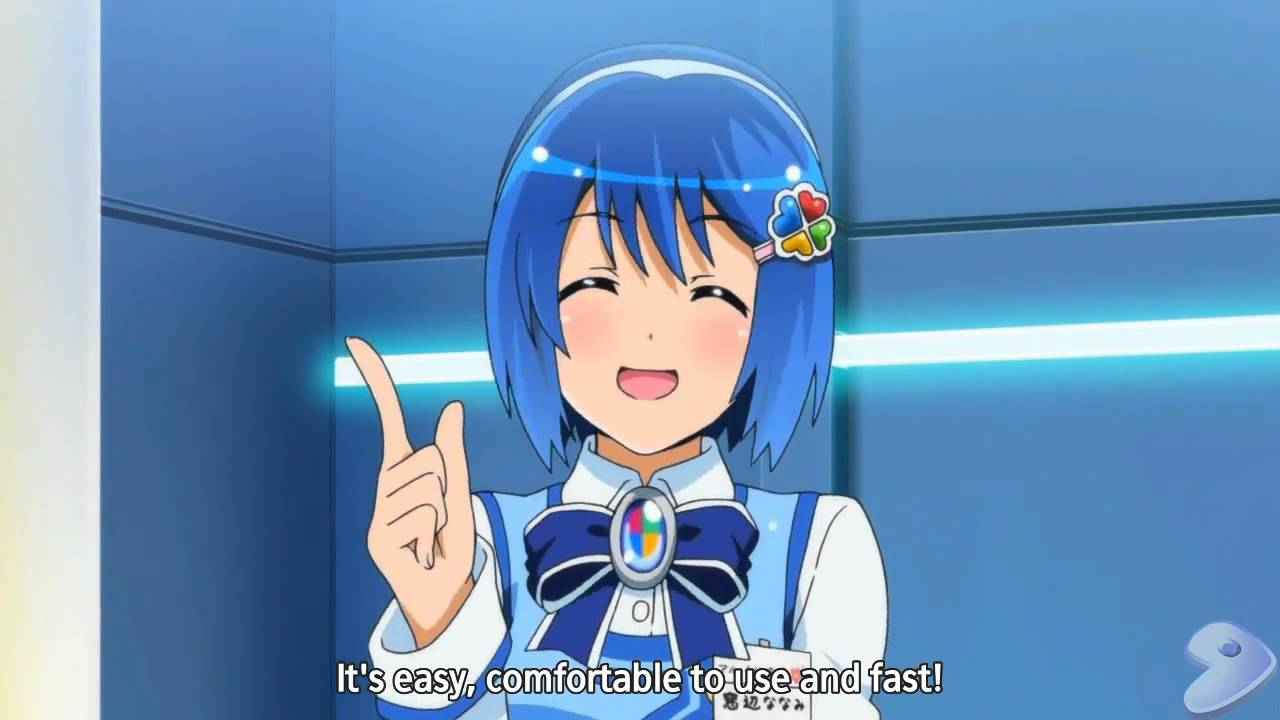
\includegraphics[width=\columnwidth]{img/nanami.jpg}
  \caption{Nanami Madobe, maskot Windows 7}
\end{figure}

Gambar dengan gaya anime umumnya digunakan dalam sektor hiburan. Salah satu bentuk penggunaan gaya anime adalah dalam pembuatan persona di internet. Persona ini digunakan untuk melakukan aktivitas publik menggunakan identitas samaran, umumnya untuk membuat video hiburan. Saat ini, salah satu sektor yang banyak digemari adalah \textit{vtuber} atau \textit{virtual youtuber}, dimana seseorang menggunakan teknologi pengenalan wajah untuk menggerakan gambar karakter bergaya anime dan memberikan kesan gambar menjadi hidup.

\begin{figure}[ht]
  
\includegraphics[width=\columnwidth]{img/kobo.jpg}
  \caption{Kobo Kanaeru, \textit{vtuber} asal Indonesia yang berada dalam naungan agensi Hololive}
\end{figure}

Teknologi pengolahan dan interpretasi citra yang ada saat ini mampu mengenali wajah serta \textit{landmark} wajah menggunakan citra wajah sebagai masukan. Namun, pengenalan wajah umumnya hanya digunakan pada wajah manusia. Dalam makalah ini, akan dibahas mengenai pengenalan \textit{landmark} wajah pada gambar karakter bergaya anime.

\section{Studi Literatur}
\subsection{Citra}
Menurut \cite{gonzalez2009digital}, sebuah citra dapat didefinisikan sebagai fungsi dwimatra $f(x, y)$ dengan $x, y$ adalah koordinat spasial dan keluaran fungsi $f$ adalah intensitas atau tingkat keabuan pada titik $x, y$. Umumnya, citra digital memiliki koordinat $x, y$ yang diskrit. Citra diskrit pada ranah digital didapatkan dengan melakukan penerokan terhadap citra pada titik-titik tertentu, lalu melakukan kuantisasi dari nilai-nilai tingkat keabuan yang diterok. Hasil penerokan memberikan citra yang dapat direpresentasikan sebagai matriks dengan $M$ baris dan $N$ kolom seperti pada persamaan~\ref{citramatrix}.

\begin{multline}
  \label{citramatrix}
  f(x,y) = \\
  \left[
    \begin{matrix}
      f(0, 0)   & f(0, 1)   & \cdots & f(0, N-1)   \\
      f(1, 0)   & f(1, 1)   & \cdots & f(1, N-1)   \\
      \vdots    & \vdots    &        & \vdots      \\
      f(M-1, 0) & f(M-1, 1) & \cdots & f(M-1, N-1)
    \end{matrix}
    \right]
\end{multline}

Untuk sembarang citra, proses kuantisasi memetakan tingkat keabuan pada sejumlah $L$ tingkat keabuan yang mungkin ada. Tingkat diskrit pada $L$ dapat diasumsikan merupakan bilangan bulat yang tersebar merata dalam interval $[0, L-1]$. Umumnya, $L$ merupakan suatu pangkat bilangan bulat dari 2: $L = 2^k$.

Citra yang berwarna dapat direpresentasikan dengan menyimpan tingkat keabuan untuk tiga warna dasar, yakni merah (R), hijau (G), dan biru (B).

\subsection{Warna}
Warna yang dapat direspon oleh mata manusia memiliki panjang gelombang antara \qty{400}{\nano\meter} hingga \qty{700}{\nano\meter}. Terdapat tiga warna yang memiliki kombinasi rentang terbesar, yakni merah, hijau, dan biru. Ketiganya seringkali disebut sebagai warna pokok. Warna-warna lain dapat dihasilkan dengan menggabungkan ketiga warna pokok dengan perbandingan tertentu.

Terdapat beberapa model warna yang terdefinisi. Model warna yang umumnya digunakan untuk penyimpanan dan pengolahan antara lain model warna RGB, CMYK, serta YCbCr. Model warna RGB menggunakan warna pokok seperti yang disebutkan sebelumnya. Model warna CMYK menggunakan warna sekunder yang dihasilkan dari penggabungan merah, hijau, dan biru, dengan tambahan warna hitam sebagai key. Model warna YCbCr menggunakan kecerahan serta kroma pada warna biru dan merah.

Selain model warna untuk penyimpanan dan pengolahan, terdapat pula model warna yang merepresentasikan pengalaman indera manusia secara lebih baik. Model warna tersebut adalah HSV, yang memisahkan warna, kecerahan, dan saturasi. Dalam model warna HSV, warna dikodekan sebagai \textit{hue}, \textit{saturation}, dan \textit{value}. Nilai \textit{hue} merepresentasikan warna dalam rentang $[0, 2\pi]$. Nilai \textit{saturation} merepresentasikan kepekatan warna dalam rentang $[0,1]$. Nilai \textit{value} merepresentasikan kecerahan warna dalam rentang $[0,1]$. Ilustrasi dari model warna HSV dapat dilihat pada gambar~\ref{hsv}.

\begin{figure}[ht]
  \begin{center}
    \includestandalone[width=5cm]{diagrams/hsv}
  \end{center}
  \caption{Ilustrasi model warna HSV.}\label{hsv}
\end{figure}

\subsection{Deteksi Tepi}
Disebutkan dalam \cite{munir2022edge}, tepi merupakan salah satu fitur yang ada dalam citra. Tepi didefinisikan sebagai perubahan nilai keabuan yang besar dalam jarak spasial yang pendek. Terdapat empat macam tepi: tepi curam, tepi landai, tepi garis, dan tepi atap. Pendeteksian tepi berguna untuk meningkatkan penampakan garis batas objek, serta mengekstrasi representasi garis-garis dalam citra.

Pendeteksian tepi dapat dilakukan dengan menggunakan beberapa operator. Operator yang paling sederhana adalah operator gradien, yakni operator yang menghitung kemiringan dari fungsi. Variasi dari operator ini adalah operator gradien dengan selisih-terpusat (\textit{center-difference}).

Operator lain yang mungkin digunakan dalam pendeteksian citra adalah operator Laplace atau turunan kedua. Operator laplace menggunakan turunan kedua untuk mencari perubahan tanda gradien, yakni dengan mencari persilangan nol (\textit{zero-crossing}). Operator Laplace didapatkan dengan mengambil gradien orde kedua dari $f(x,y)$, atau menurunkan $f(x,y)$ secara diskrit sebanyak dua kali. Operator Laplacian dapat dilakukan dengan melakukan konvolusi menggunakan kernel pada persamaan~\ref{laplacian}.
\begin{equation}
  D^2_{xy} = \left [\begin{matrix}
      0 & 1  & 0 \\
      1 & -4 & 1 \\
      0 & 1  & 0
    \end{matrix}\right ]
  \label{laplacian}
\end{equation}

Derau dapat dideteksi sebagai tepi akibat perubahan nilai keabuan yang cepat. Oleh karena itu, perlu ditapis terlebih dahulu. Salah satu penapis yang mungkin digunakan adalah penapis Gaussian, yang melembutkan citra. Dalam kasus operasi Laplace, penapis Gaussian dapat digabungkan dengan operasinya. Oleh karena itu, perhitungan tepi menggunakan operasi Laplace dapat dilakukan lebih efisien. Operator Laplace yang dilengkapi dengan Gaussian umumnya disebut sebagai operator tersendiri, yakni Laplacian of Gaussian (LoG). Kernel untuk LoG didapatkan dengan menggunakan persamaan~\ref{log}.
\begin{equation}
  \mathrm{LoG}(u, v) = \frac{1}{\pi \sigma^4}
  \left(\frac{u^2 + v^2}{2\sigma^2} - 1\right)
  e^{-\frac{u^2+v^2}{2\sigma^2}}
  \label{log}
\end{equation}

Selain kedua operasi tersebut, terdapat operasi Canny yang dapat digunakan untuk mendeteksi tepi. Tepi yang dideteksi oleh operator Canny akan memiliki lebar 1 pixel, berbeda dengan operasi-operasi lainnya. Operator Canny mendapatkan tepi dengan langkah-langkah sebagai berikut:
\begin{enumerate}
  \item Haluskan citra menggunakan penapis Gaussian
  \item Hitung gradien serta arahnya menggunakan operator deteksi tepi lainnya
  \item Ambangkan nilai tepi yang didapat sebelumnya
\end{enumerate}

Pengambangan dalam operator Canny menggunakan dua nilai ambang, $T1$ dan $T2$ untuk mengklasifikasi tepi menjadi tepi kuat dan tepi lemah. jika magnitudo tepi melebihi $T2$, maka tepi tersebut diklasifikasikan menjadi tepi kuat. Apabila magnitudo tepi berada antara $T1$ dan $T2$, maka tepi tersebut diklasifikasikan sebagai tepi lemah. Di luar kasus tersebut, maka dianggap sebagai bukan tepi. Hasil dari operator Canny merupakan tepi kuat serta tepi lemah yang berhubungan dengan tepi kuat.

\subsection{Kontur}
Menurut \cite{munir2022kontur}, kontur merupakan serangkaian tepi yang membentuk batas daerah tertentu. Kontur dapat direpresentasikan sebagai senarai tepi (\textit{edge list}) atau berupa kurva. Kode rantai dapat digunakan untuk mengkodekan senarai tepi.

Pencocokan kurva dalam tepi dapat dilakukan dengan melakukan interpolasi dan penghampiran. Salah salah satu metode untuk melakukan penghampiran kurva pada tepi adalah transformasi Hough. Teknik tersebut dapat menghampiri kurva parametrik dalam tepi.

Transformasi Hough menggunakan bentuk parametrik kurva untuk melakukan penghampiran. Kemudian, mekanisme yang dilakukan untuk mengestimasi nilai parameter adalah dengan pemungutan suara untuk setiap kombinasi parameter. Setiap titik tepi memberikan suara untuk kombinasi parameter tertentu. Parameterisasi untuk garis lurus dapat dilakukan dengan mengubah persamaan garis lurus $y = mx + c$ ke dalam ruang parameter m - c: $c = y - mx$. Namun, kelemahan ruang parameter ini adalah adanya nilai gradien $m$ yang tidak terdefinisi untuk garis tegak lurus. Oleh karena itu, alternatif parameterisasi yang mungkin dilakukan adalah dengan mengubah persamaan garis ke bentuk normal Hesse, yakni $r = x \cos \theta + y \sin \theta$. Transformasi Hough memberikan nilai kemungkinan adanya garis dengan parameter dalam ruang parameter. Garis yang didekati dapat diambil berdasarkan nilai ambang untuk jumlah suara tertentu. Visualisasi hasil transformasi Hough untuk citra tertentu dapat dilihat pada gambar~\ref{hough}.

\begin{figure}
  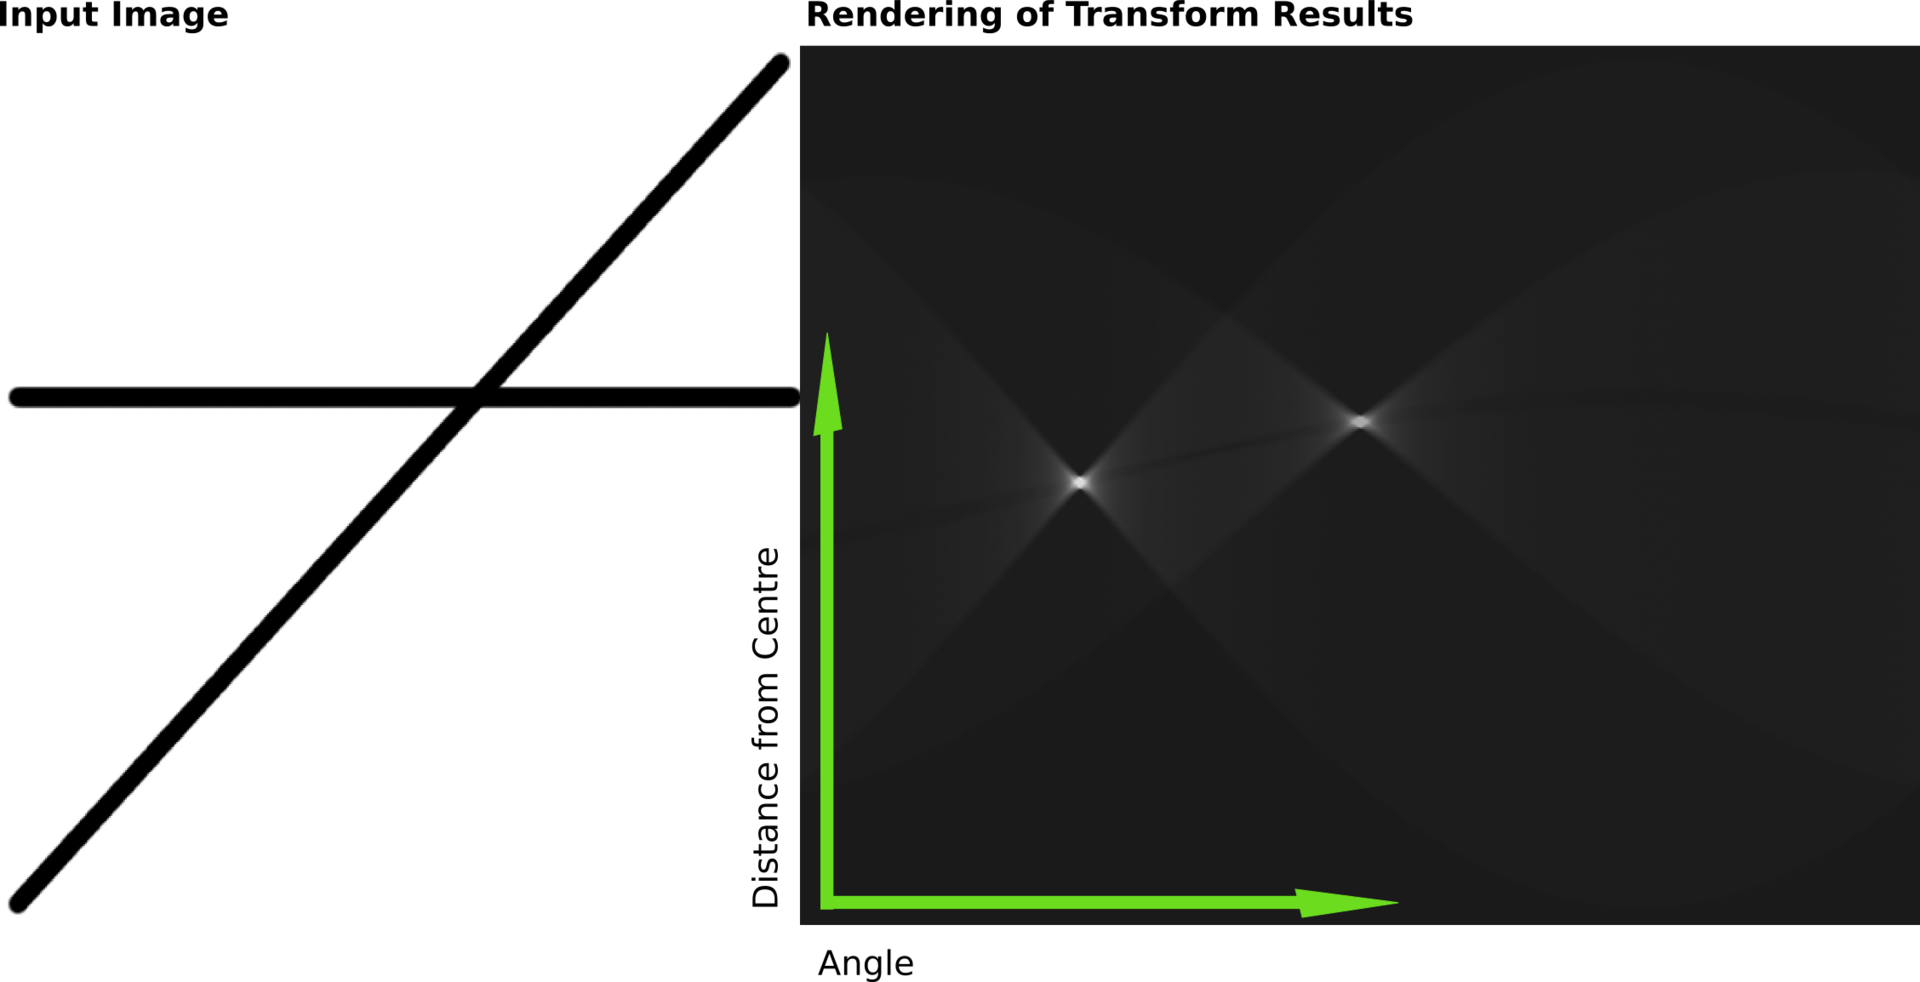
\includegraphics[width=\columnwidth]{img/hough_ex.png}
  \caption{Contoh hasil transformasi Hough untuk citra dengan 2 garis tebal. Diambil dari Wikipedia}\label{hough}
\end{figure}

\subsection{Segmentasi}
Suatu citra dapat disegmentasi menjadi beberapa bagian, berdasarkan kriteria tertentu. Segmentasi dapat berguna untuk memisahkan objek yang ingin diproses dengan hal di sekitarnya. Umumnya teknik segmentasi citra dapat dikelompokkan menjadi dua pendekatan, yakni berbasis diskontinuitas serta berbasis kesamaan.

Pendeteksian segmen menggunakan kesamaan salah satunya dapat dilakukan dengan pengambangan. Pada citra orang atau karakter anime, umumnya terdapat warna kulit yang diterima agar dapat didefinisikan sebagai karakter. Oleh karena itu, segmentasi dapat dilakukan dengan melakukan pengambangan pada model warna HSV.

Selain menggunakan pengambangan, segmen dapat dibangun menggunakan algoritma \textit{K-Means}. Algoritma \textit{K-Means} merupakan algoritma yang dapat mengelompokkan data menjadi $k$ kelompok berdasarkan ukuran kemiripan yang diberikan. Penggunaan algoritma \textit{K-Means} adalah untuk mensegmentasi citra menjadi beberapa segmen warna.

\section{Studi Terkait}
Dalam \cite{takayama2012face}, dideskripsikan cara untuk mendeteksi wajah karakter kartun menggunakan teknik-teknik pengolahan citra. Dalam studi tersebut, digunakan nilai \textit{hue} tertentu untuk mendeteksi wajah berdasarkan warna kulit. Nilai rentang \textit{hue} yang digunakan adalah $[0, 40]$ dalam derajat. Selain itu, faktor \textit{value} juga digunakan dalam untuk mendeteksi warna kulit. Nilai rentang yang digunakan adalah $[0.75, 1]$.

\section{Implementasi Solusi}
Solusi dibuat menggunakan bahasa pemrograman \texttt{Python} versi 3.9. Pustaka \texttt{OpenCV} versi 4.6 serta \texttt{NumPy} digunakan untuk membantu melakukan berbagai operasi pada citra secara efisien. Alur umum solusi dapat dilihat pada gambar~\ref{sol}.

\begin{figure}[ht]
  \includestandalone[width=\columnwidth]{diagrams/solution_flow}
  \caption{Diagram alur solusi}\label{sol}
\end{figure}

Masukan dari prrogram adalah sebuah citra yang berisi wajah karakterr anime. Keluaran dari program adalah titik-titik yang membentuk kontur wajah serta titik \textit{landmark} berupa dua buah titik mata dan satu buah titik dagu.

Proses pertama yang dilakukan oleh program adalah melakukan segmentasi gambar untuk mengekstraksi bagian yang berisi warna kulit. Berdasarkan penelitian \cite{takayama2012face}, nilai \textit{hue} yang cocok menjadi batas ambang adalah $40$. Namun, berdasarkan eksperimen, nilai ambang $60$ menghasilkan segmentasi yang lebih baik. Selain itu, hasil segmentasi menghasilkan pixel-pixel putih yang tidak diinginkan, sehingga pixel-pixel putih dibuang. Hasil segmentasi kemudian dideteksi tepinya. Dalam solusi yang dibuat, Segmentasi berdasarkan warna digunakan untuk mengurangi tepi-tepi yang tidak digunakan. Citra yang digunakan sebagai contoh dapat dilihat pada gambar~\ref{im1}. Visualisasi hasil segmentasi kulit dapat dilihat pada gambar~\ref{skinsep}. Visualisasi hasil pendeteksian tepi dapat dilihat pada gambar~\ref{skinedges}.

\begin{figure}[ht]
  \begin{center}
    
\includegraphics[width=6cm]{img/hatsune_miku.jpg}
  \end{center}
  \caption{Citra Hatsune Miku yang digunakan untuk percobaan}\label{im1}
\end{figure}

\begin{figure}[ht]
  \begin{center}
    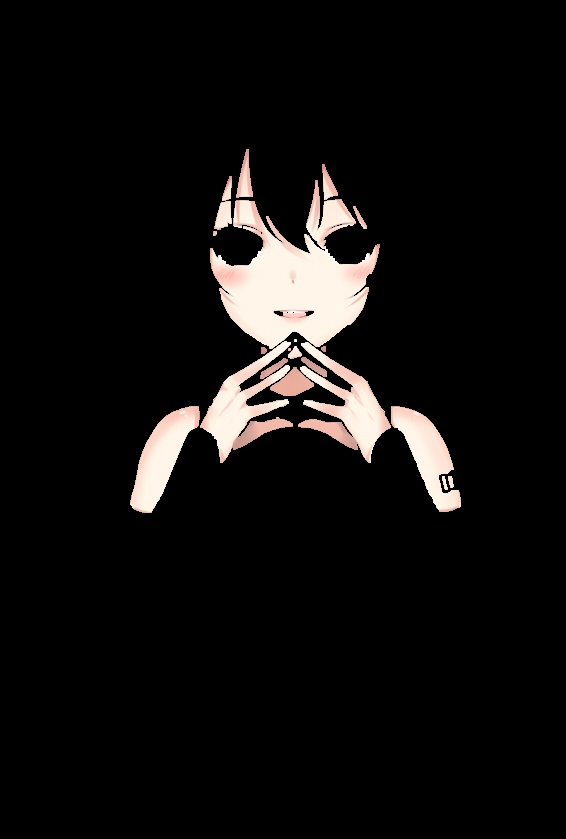
\includegraphics[width=6cm]{img/process_skin_threshold.jpg}
  \end{center}
  \caption{Visualisasi ekstraksi warna kulit}\label{skinsep}
\end{figure}
\begin{figure}[ht]
  \begin{center}
    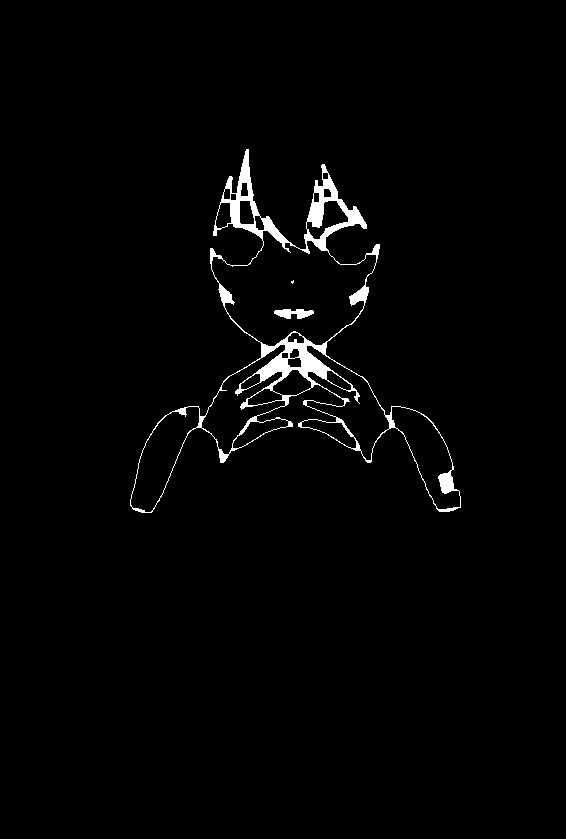
\includegraphics[width=6cm]{img/process_skin_edges.jpg}
  \end{center}
  \caption{Visualisasi pendeteksian tepi pada segmen kulit}\label{skinedges}
\end{figure}

Selanjutnya, untuk setiap daerah atau kontur tertutup, dilakukan pencocokan menggunakan transformasi Hough. Pencocokan garis dilakukan untuk mencari garis-garis yang membangun wajah. Berdasarkan observasi, garis yang membangun wajah pada karakter anime relatif lurus. Kemudian, terdapat garis yang bertemu pada titik dagu. Oleh karena itu, pendeteksian dagu dilakukan dengan mencari dua buah pasangan titik yang bertemu pada titik di dalam segmen pada rentang sudut tertentu. Dari eksperimen, didapatkan rentang sudut yang cukup optimal untuk wajah yang menghadap depan adalah $[50, 100]$ dalam derajat. Namun, rentang tersebut mungkin berubah tergantung pada gaya penggambaran spesifik yang digunakan. Visualisasi garis hasil transformasi Hough pada salah satu kontur dapat dilihat pada gambar~\ref{viz_hough}.

\begin{figure}[ht]
  \begin{center}
    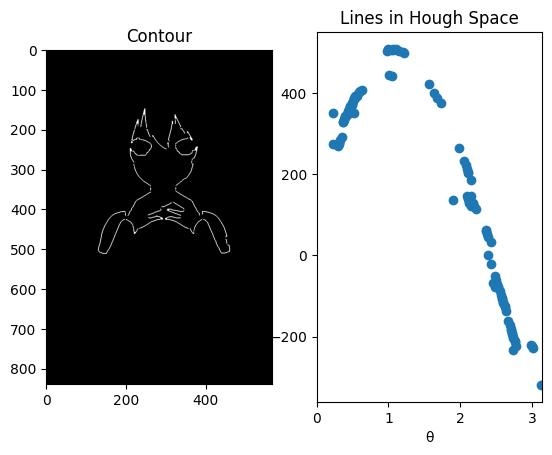
\includegraphics[width=\columnwidth]{img/process_hough_1.jpg}
  \end{center}
  \caption{Visualisasi transformasi Hough untuk kontur}\label{viz_hough}
\end{figure}

Setelah mendapatkan kontur yang mungkin berisi wajah beserta titik dagu, mata akan dicari dalam kontur tersebut. Pencarian mata dilakukan dengan pertama-tama melakukan segmentasi berdasarkan warna pada bagian wajah menggunakan algoritma \textit{K-Means}. Berdasarkan eksperimen, nilai K yang optimal adalah 3, karena umumnya dalam wilayah wajah, tidak banyak warna selain warna kulit dan warna rambut. Visualisasi hasil segmentasi menggunakan \textit{K-Means} dapat dilihat pada gambar~\ref{kmeans}. Dari hasil segmentasi, diambil segmen dengan jumlah pixel paling sedikit. Visualisasi segmen dengan jumlah pixel paling sedikit dapat dilihat pada gambar~\ref{eye_cluster}.

\begin{figure}[ht]
  \begin{center}
    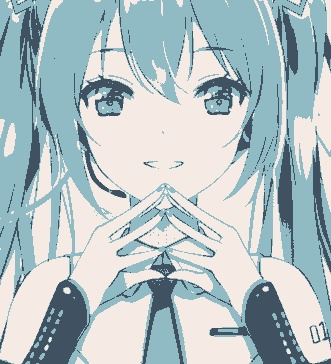
\includegraphics[width=5cm]{img/process_seg_kmeans.jpg}
  \end{center}
  \caption{Visualisasi hasil \textit{K-Means} dengan $k=3$}\label{kmeans}
\end{figure}

\begin{figure}[ht]
  \begin{center}
    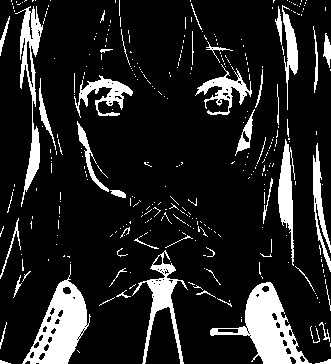
\includegraphics[width=5cm]{img/process_eye_candidates.jpg}
  \end{center}
  \caption{Visualisasi segmen yang mungkin mencakup mata}\label{eye_cluster}
\end{figure}

Berdasarkan observasi, umumnya mata pada karakter anime memiliki \textit{outline} yang umumnya berwarna gelap, serta simetris antara kanan dan kiri. Oleh karena itu, akan dicari komponen dengan kontur yang memiliki bentuk yang mirip. Selain memiliki bentuk yang mirip, umumnya mata juga memiliki warna yang sama, maka akan dicari segmen yang memiliki warna yang mirip. Dalam eksperimen, didapaatkan nilai kemiripan berada di bawah ambang $(45, 65, 40)$ dalam model warna HSV. Visualisasi hasil pasangan mata yang didapatkan dapat dilihat pada gambar~\ref{eyes}.

\begin{figure}[ht]
  \begin{center}
    
\includegraphics{img/eye_candidate_1.jpg}
    
\includegraphics{img/eye_candidate_2.jpg}
  \end{center}
  \caption{Visualisasi pasangan mata yang didapatkan}\label{eyes}
\end{figure}

Setelah mata didapatkan, maka proses akhir adalah dengan mengambil titik tengah dari \textit{bounding box} segmen mata, untuk mengaproksimasi posisi mata. Visualisasi hasil akhir dari solusi dapat dilihat pada gambar~\ref{landmark}. Visualisasi hasil akhir memberikan \textit{bounding box} wajah yang ditemukan dalam persegi berwarna hijau dan \textit{landmark} ditandai dengan titik berwarna merah.

\begin{figure}[ht]
  \begin{center}
    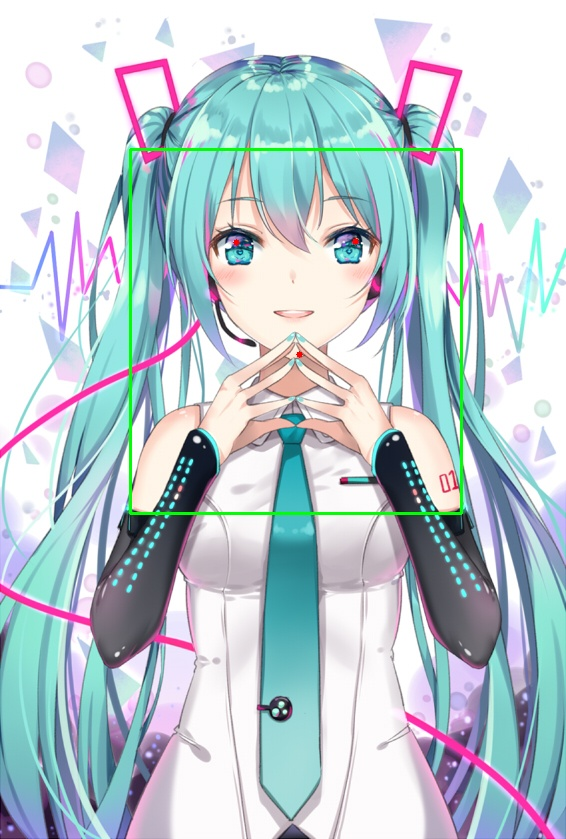
\includegraphics[width=6cm]{img/result.jpg}
  \end{center}
  \caption{Visualisasi titik-titik \textit{landmark}}\label{landmark}
\end{figure}

\section{Pengujian}
Citra lain digunakan untuk menguji kebenaran solusi yang diberikan. Citra yang akan digunakan dapat dilihat pada gambar~\ref{extratests}. Citra tambahan tidak diproses terlebih dahulu sebelumnya, dan hasilnya dapat dilihat pada gambar~\ref{extrares}.

\begin{figure}[h]
  \begin{center}
    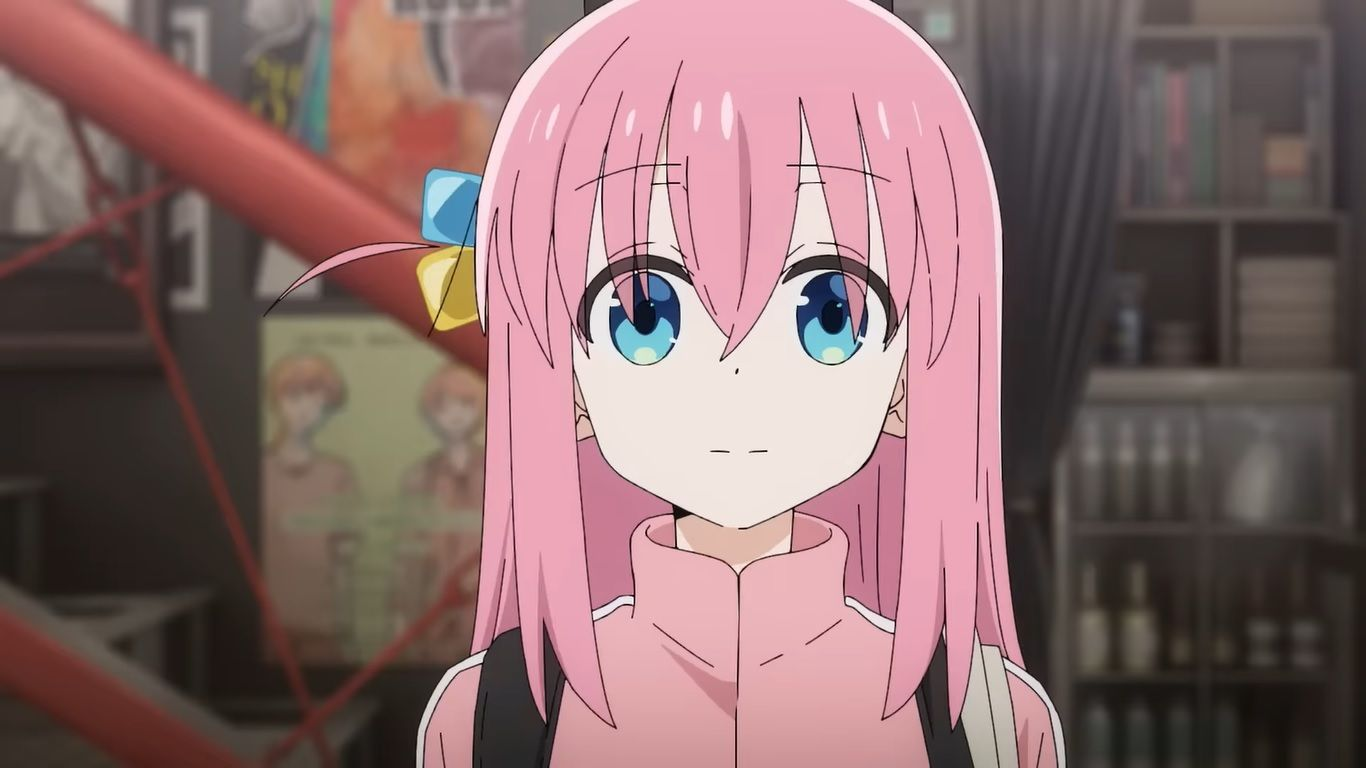
\includegraphics[width=6cm]{img/bocchi.jpg}
    
\includegraphics[width=6cm]{img/venti.jpg}
    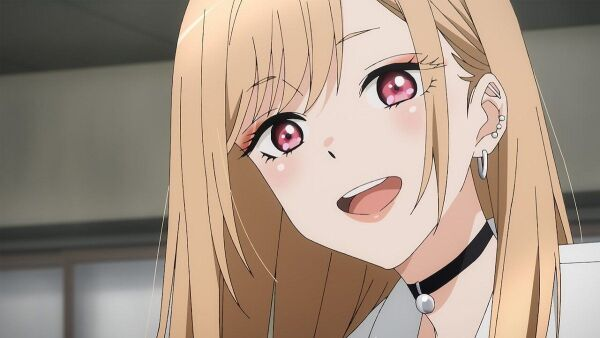
\includegraphics[width=6cm]{img/marin.jpg}
  \end{center}
  \caption{Citra uji tambahan}\label{extratests}
\end{figure}

\begin{figure}[h]
  \begin{center}
    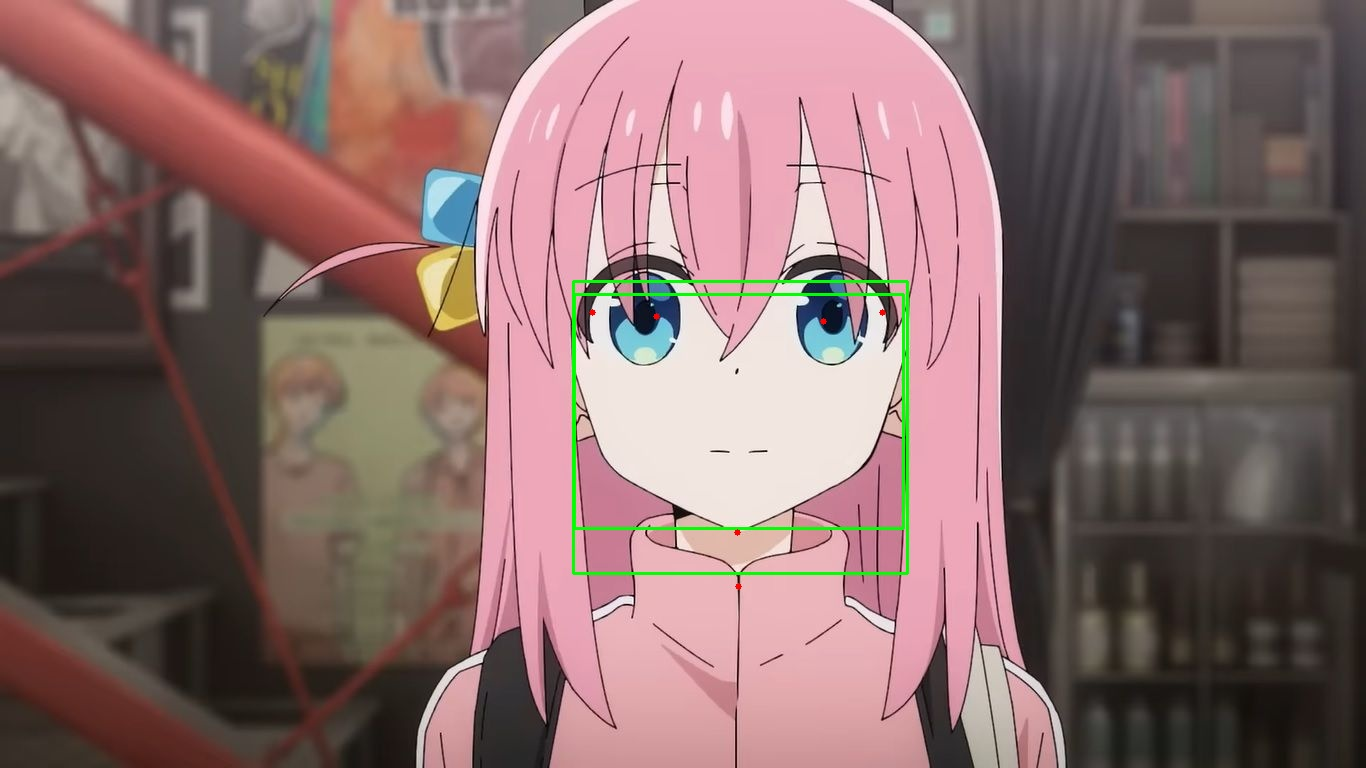
\includegraphics[width=6cm]{img/result_bocchi.jpg}
    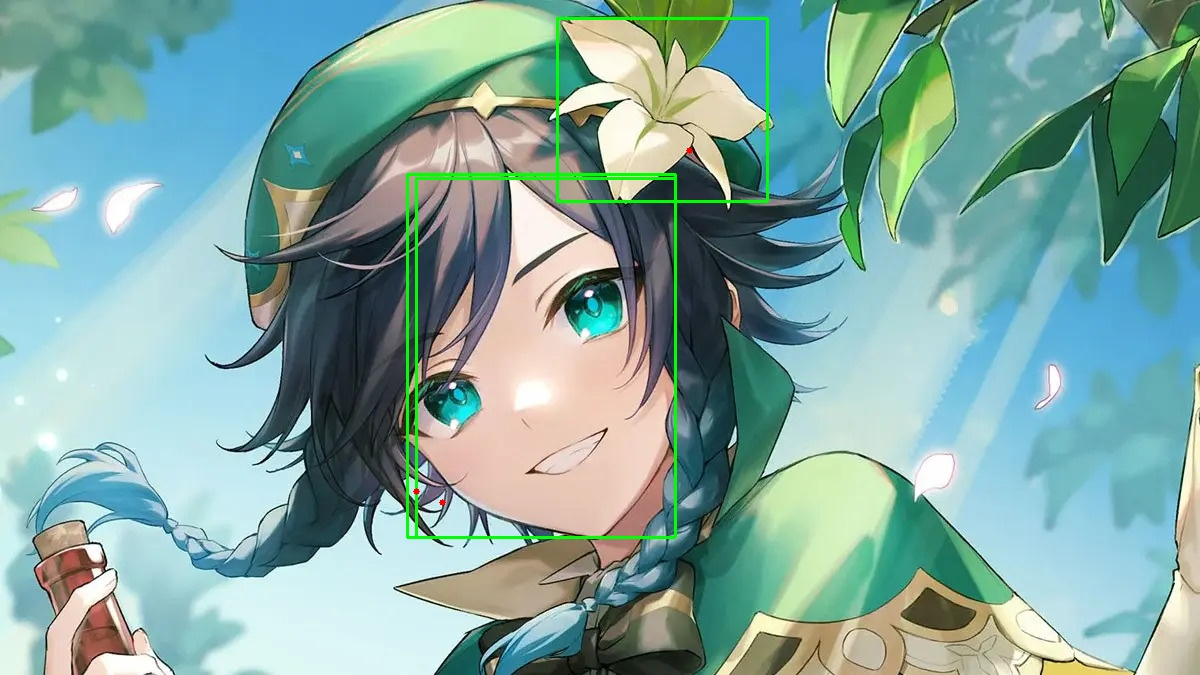
\includegraphics[width=6cm]{img/result_venti.jpg}
    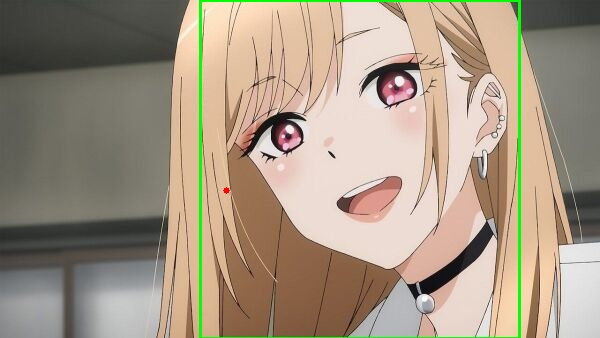
\includegraphics[width=6cm]{img/result_marin.jpg}
  \end{center}
  \caption{Hasil pengujian pada citra uji tambahan}\label{extrares}
\end{figure}

\section{Kesimpulan dan Saran}
\subsection{Kesimpulan}
Hasil dari pengujian menunjukkan masih banyak kesalahan pendeteksian wajah. Dari titik-titik yang didapatkan, kemungkinan kesalahan terjadi pada saat pendeteksian dagu. Karena posisi dagu yang tidak diketahui, maka sulit untuk menentukan apakah dua buah garis yang bersilangan membangun dagu atau tidak. Hal tersebut mempengaruhi pendeteksian mata yang dilakukan, karena pendeteksian mata didasarkan pada kemiripan jarak antara mata dengan dagu.

\subsection{Saran}
Penggunaan kakas yang lebih canggih seperti \textit{Haar Cascade Classifier} dapat mempercepat proses pencarian \textit{landmark} wajah maupun pendeteksian wajah itu sendiri. Menggunakan \textit{cascading classifier}, pencarian pola dapat dilakukan dengan lebih efektif dibandingkan \textit{brute-force}.

\section*{Pranala Terkait}
 {
  \setlength{\parindent}{0pt}
  Repository GitHub: \url{https://github.com/suggoitanoshi/if4073-pengenalan-anime}
 }

\section*{Ucapan Terima Kasih}
Syukur kepada Tuhan Yang Maha Esa atas karunia-Nya sehingga penulis dapat menyelesaikan makalah ini tanpa kesulitan maupun tantangan yang terlalu berat. Terima kasih yang teramat banyak kepada Bapak Rinaldi selaku dosen pengampu mata kuliah IF4073 Interpretasi dan Pengolahan Citra, sehingga penulis dapat belajar lebih lanjut mengenai citra dan pengolahannya. Ucapan terima kasih juga diberikan kepada keluarga dan teman-teman yang senantiasa membantu dan memberikan semangat kepada penulis sehingga penulis tidak menyerah dalam menyelesaikan perkuliahan di semester ini.

\bibliographystyle{ieeetr}
\bibliography{references}
\vspace{12pt}

\section*{Pernyataan}
\noindent
Dengan ini saya menyatakan bahwa makalah yang saya tulis ini adalah tulisan saya sendiri, bukan saduran, atau terjemahan dari makalah orang lain, dan bukan plagiasi.

  {
    \raggedleft

    Bandung, 16 Desember 2022

    \includegraphics[width=4cm, right]{img/tandatangan.png}
    Fransiskus Febryan Suryawan\\
    13519124\\
  }

\end{document}
